\setchapterpreamble[u]{\margintoc}
\glsresetall % reset glossary
\chapter{Optimizing the layout of the modules in space}
\todo{tables always small}
Introduction

\section{Optimize the modules' layout using a modified DMO algorithm}

\todo{difference with tugilimana, we take into account the buckling whensolving the first subproblem of module layout, we can have an empty subdomain andwe use a gradeint descent algo}
\begin{figure*}
    \centering
    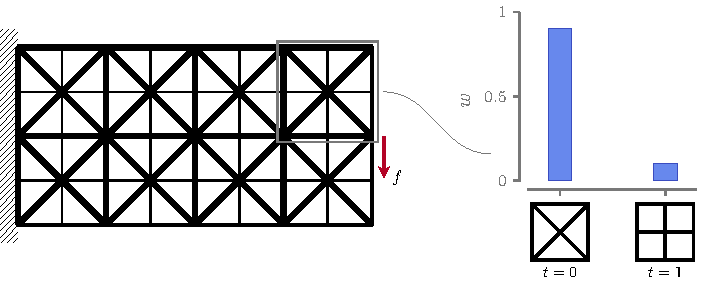
\includegraphics{figures/06_DMO/00_weight_dmo/weight_dmo.pdf}
    \caption{}
    \label{fig:06}
\end{figure*}

\subsection{Variables penalization schemes}
describe RAMP with paper of Lund. we use it because the derivative it is not infinite on alpa=0

multi-phase versions of the well-known RAMP scheme (Hvejsel and Lund, 2011)

\begin{figure}
    \centering
    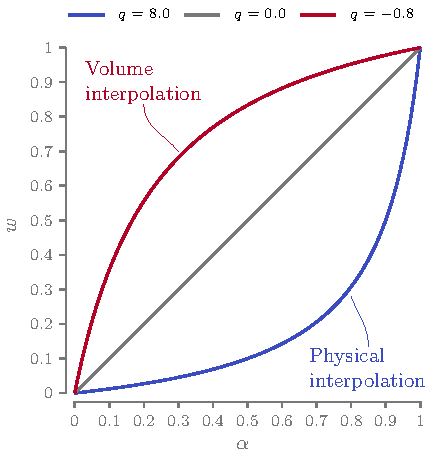
\includegraphics{figures/06_DMO/00_ramp/ramp.pdf}
    \caption{}
    \label{fig:06}
\end{figure}

multiple penalizations

continuation scheme only on p (we use an interior point algo, we want to stay in the fesable region)


\subsection{Modified DMO algorithm}
we use a dmo like approach
PRO:
Optimize a discrete problem using continuous variables
Gradient-based optimization

CONS:
Convergence of the weight to 0000100 solution FOR EVERY ELEMENT
Many optimization variables

difference with the original DMO; we are not only changing the weights but also the modules topology. Tihis is more difficoult
\paragraph*{Penalized volume}
\begin{equation}
    V = \sum_{j=1}^{N_{\text{sub}}}\vect{\bar{\ell}}^T\tilde{\vect{a}}^j
\end{equation}
\begin{equation}
    \tilde{\vect{a}}^j = \sum_{t=1}^{N_T} \tilde{w}_t^j \bar{\vect{a}}_t 
\end{equation}
and where
\begin{equation}
    \tilde{w}_t^j = \frac{\alpha_t^j}{1+q(1-\alpha_t^j)}    
\end{equation}

\begin{equation}
    \vect{a}^j = \sum_{t=1}^{N_T} w_t^j \bar{\vect{a}}_t 
\end{equation}
and where
\begin{equation}
    w_t^j = \frac{\alpha_t^j}{1+p(1-\alpha_t^j)}    
\end{equation}

\begin{equation}
    \sum_{t=1}^{N_T} w_t^j = 1
\end{equation}

\begin{equation}
    V = \sum_{j=1}^{N_{\text{sub}}}\vect{\bar{\ell}}^T\sum_{t=1}^{N_T} \frac{\alpha_t^j}{1+q(1-\alpha_t^j)} \bar{\vect{a}}_t
\end{equation}

\subsection{Optimization formulation and resolution algorithm}
\begin{equation}
    \begin{aligned}
    \min_{\bar{\vect{a}}, \vect{\alpha}, \bm{q}, \bm{U}}   && V &= \sum_{j=1}^{N_{\text{sub}}}\vect{\bar{\ell}}^T\tilde{\vect{a}}^j && \textrm{(Volume minimization)}\\
    \textrm{s.t.}   && \bm{B}\bm{q} &= \bm{f} && \textrm{(Force equilibrium)}\\
                    && \bm{q} &= \frac{\bm{a}\bm{E}}{\bm{\ell}}\bm{b}^T\bm{U} && \textrm{(Compatibility constraints)} \\
                    && \bm{q} &\geq -\frac{\bm{s}\bm{a}^2}{\bm{\ell^2}} && \textrm{(Euler buckling constraints)} \\
                    && -\sigma_C\bm{a} &\leq \bm{q} \leq \sigma_T\bm{a} && \textrm{(Stress constraints)} \\
                    && 0 &\leq \bar{\vect{a}} \leq \frac{4 \pi \bar{\vect{\ell}}^2}{\lambda_{\text{max}}} && \textrm{(Slenderness limit)} \\
                    && \sum_{t=1}^{N_T} \alpha_t^j &\leq 1, \; \forall j && \textrm{(One selected module max.)} \\
    \end{aligned}
\end{equation}

Solved using the two step algorithm, so before relaxed problem where we solve without compatibility constraints. this time, as the problem is nonlinear due to the alpha design variables, we solve it without linearizing the buckling constraints.  here is the formulation of the first subproblem:

Then the compatibility constraints are added again
we solve it fixing the submodules topology and using the VL formulation already used in \dots

hree is the schema of the solving algo:


\subsection{Optimization initialization: a clustering algorithm to identify similarly behaving subdomains}
we are not only changing the weights but also the modules topology. Tihis is more difficoult. the layout is dependent on the module topology and vice versa. so we give a slighltly influenced departure point x0. In this work we decided to infuence the weight distribuition as follows:
\begin{equation}
    \alpha_{t,\text{it}=0}^j=
    \begin{cases}
        \frac{1}{N_\text{T}} \cdot 1.1  & \text{if the $j$-th subdomain has the  $t$-th module selected,}\\
        \frac{N_\text{T}-1.1}{N_\text{T}(N_\text{T}-1)} & \text{otherwise.} \\
    \end{cases}  
\end{equation}

\begin{figure*}
    \centering
    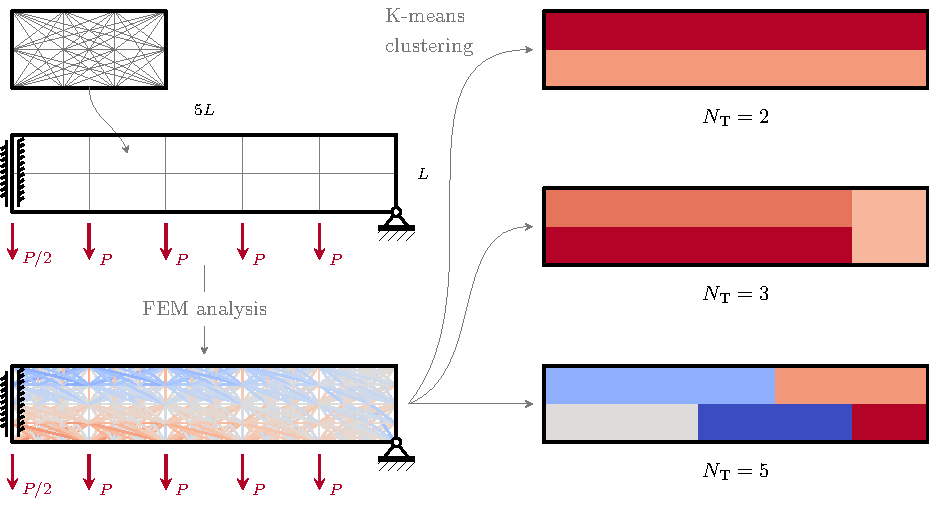
\includegraphics{figures/06_DMO/00_stress_clustering/stress_clustering.pdf}
    \caption{}
    \label{fig:06}
\end{figure*}

\begin{figure*}
    \centering
    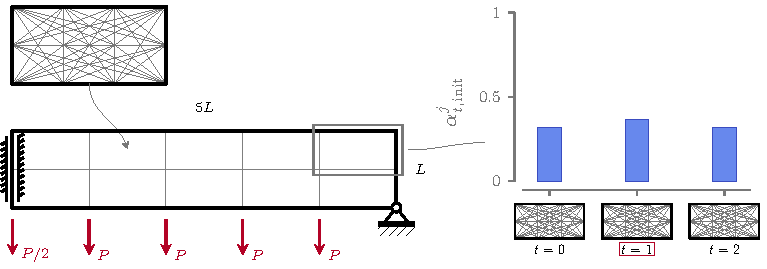
\includegraphics{figures/06_DMO/00_x0/x0.pdf}
    \caption{}
    \label{fig:06}
\end{figure*}

the initial layout of modules is assessed using a k meeans clustering technique with nt clusters. Given a set of observations (x1, x2, ..., xn), where each observation is a d-dimensional real vector, k-means clustering aims to partition the n observations into n sets. we define the observation as the vector containing the stress of the bars of unoptimized initial ground structure plus the stress state S For the j-th submodule we define the 

\begin{equation}
    S^j=\sum_{i=0}^{\bar{n}}|\sigma^j_i|
\end{equation}
This add permits to promote the clustering of not only submodules loaded in similar ways, but also on similar magnitude (and have so more voluminous and less voluminous modules).

\section{Numerical application}
IPOPT for the two steps
\subsection{Layout optimization of fixed modules}
\begin{marginfigure}
    \centering
    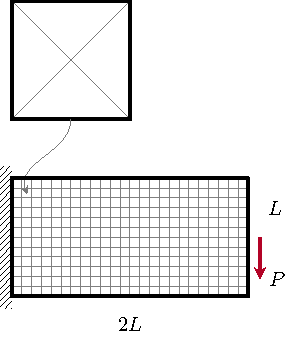
\includegraphics[width=\linewidth]{figures/06_DMO/00_cantilever_bcs/cant_mesh.pdf}
    \caption{Boundary conditions of the 2D cantilever beam divided in 24x12 subdomains. In the upper part of the image the ground structure of the module composed of $\bar{n}=6$ elements.}
    \label{fig:06_cant_BC_GS}
\end{marginfigure}
\begin{margintable}
    \small
    \centering
    \begin{tabular}{cc}
    \toprule
    \textbf{Parameter}        & \textbf{Value} \\ \midrule
    $L$              & 100     \\
    $\sigma_\text{c}, \sigma_\text{t}$ & $\pm 1$\\
    $P$              & 1   \\
    $a_\text{max}$              & 0.6   \\
    \bottomrule
    \end{tabular}
    \caption{Material data used for the 2D cantilever beam 2D.}
    \label{tab:06_modular_cant_data}
\end{margintable}
\begin{figure*}
    \subcaptionbox{}{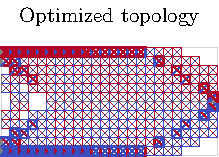
\includegraphics{figures/06_DMO/00_fixed_cells/top_00.pdf}}
    \hfill
    \subcaptionbox{}{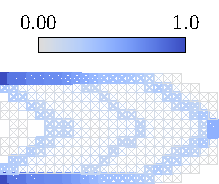
\includegraphics{figures/06_DMO/00_fixed_cells/weight_00.pdf}}
    \hfill
    \subcaptionbox{}{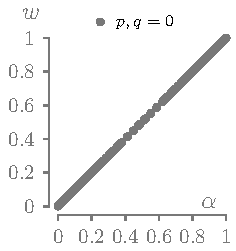
\includegraphics[height=3.5cm] {figures/06_DMO/00_fixed_cells/ramp_00.pdf}}
    \hfill
    \subcaptionbox{}{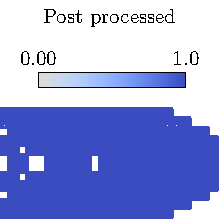
\includegraphics{figures/06_DMO/00_fixed_cells/weight_00_PP.pdf}}
    \bigskip
    \subcaptionbox{}{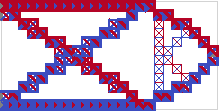
\includegraphics{figures/06_DMO/00_fixed_cells/top.pdf}}
    \hfill
    \subcaptionbox{}{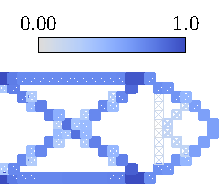
\includegraphics{figures/06_DMO/00_fixed_cells/weight.pdf}}
    \hfill
    \subcaptionbox{}{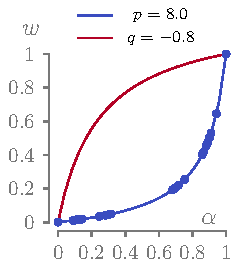
\includegraphics[height=3.5cm]{figures/06_DMO/00_fixed_cells/ramp.pdf}}
    \hfill
    \subcaptionbox{}{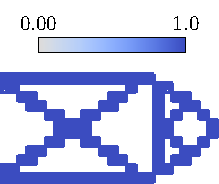
\includegraphics{figures/06_DMO/00_fixed_cells/weight_PP.pdf}}
    \caption{}
    \label{fig:06}
\end{figure*}

\begin{figure}
    \subcaptionbox{}{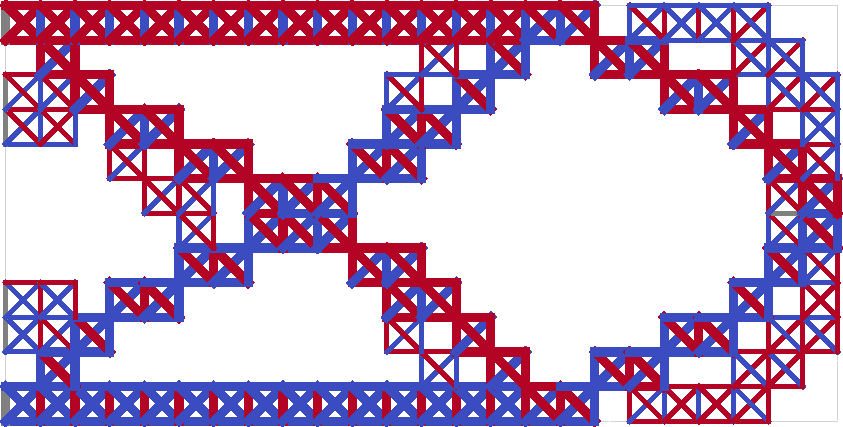
\includegraphics[width=0.45\linewidth]{figures/06_DMO/00_fixed_cells_multiple/fig1-Topology_area.pdf}}
    \hfill
    \subcaptionbox{}{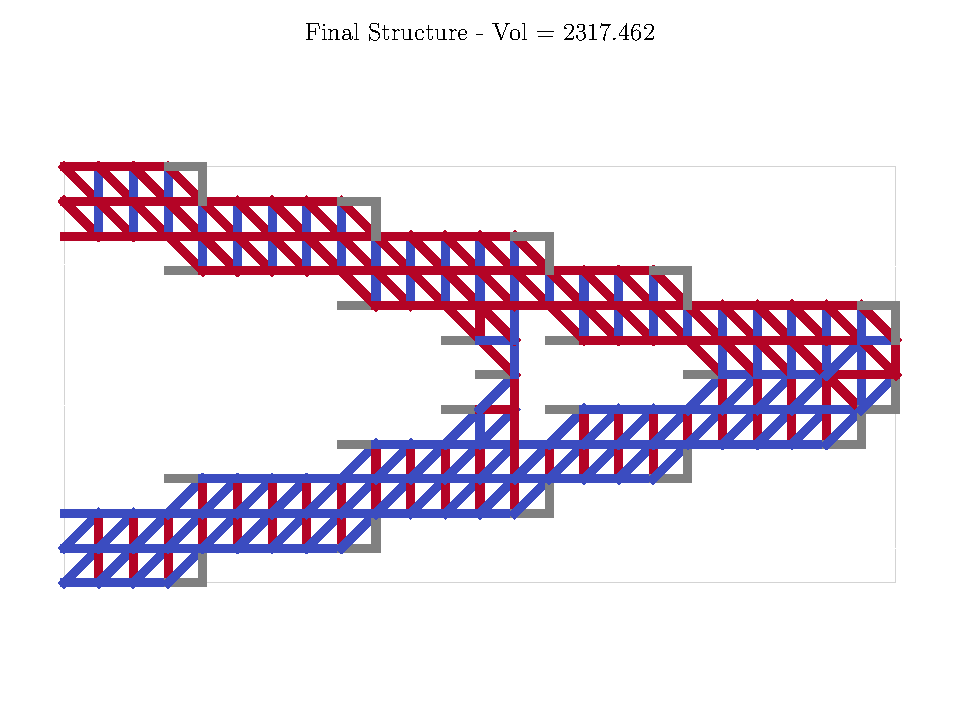
\includegraphics[width=0.45\linewidth]{figures/06_DMO/00_fixed_cells_multiple/fig1-Topology_topol.pdf}}
    \hfill
    \bigskip
    \subcaptionbox{}{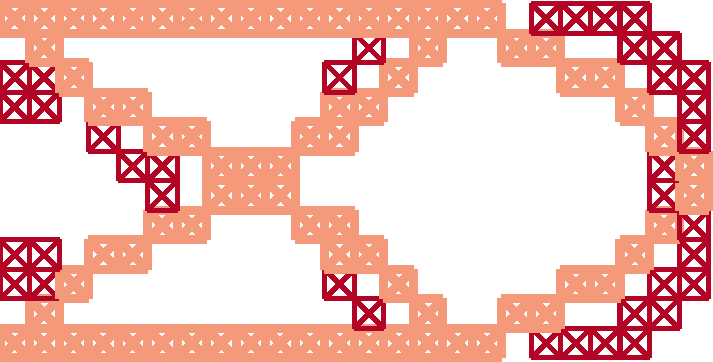
\includegraphics[width=0.45\linewidth]{figures/06_DMO/00_fixed_cells_multiple/fig12-Module_withType_area.pdf}}
    \hfill
    \subcaptionbox{}{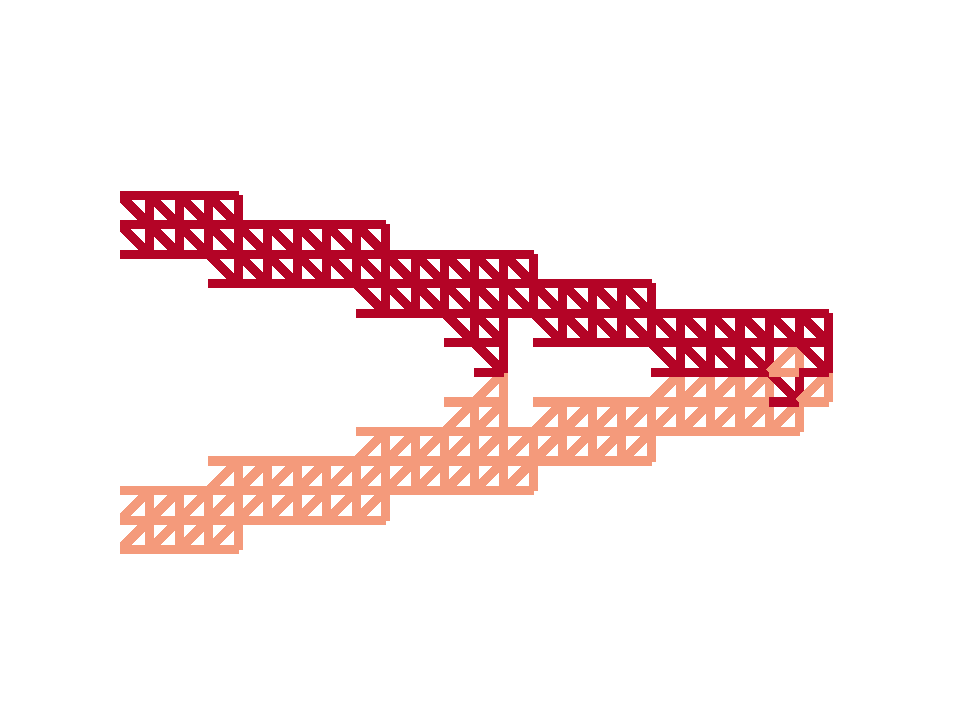
\includegraphics[width=0.45\linewidth]{figures/06_DMO/00_fixed_cells_multiple/fig12-Module_withType_topol.pdf}}
    \caption{}
    \label{fig:06}
\end{figure}
\subsection{Modules and layout optimization}
\begin{figure}
    \hspace*{\fill}
    \subcaptionbox{}{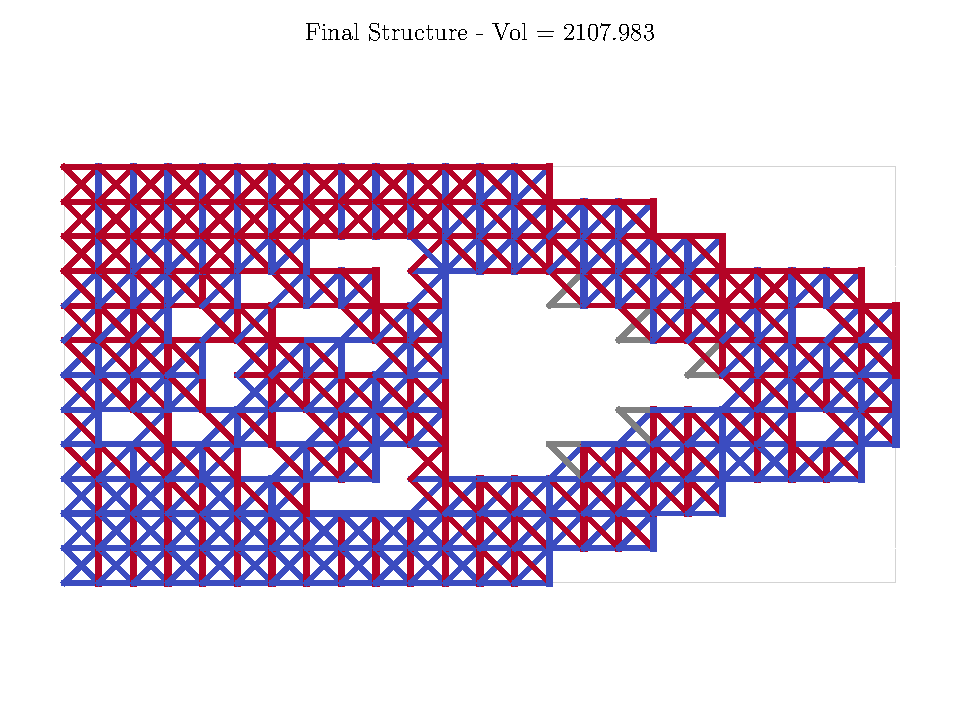
\includegraphics[width=0.45\linewidth]{figures/06_DMO/00_optimized_module/fig1-Topology.pdf}}
    \hfill
    \subcaptionbox{}{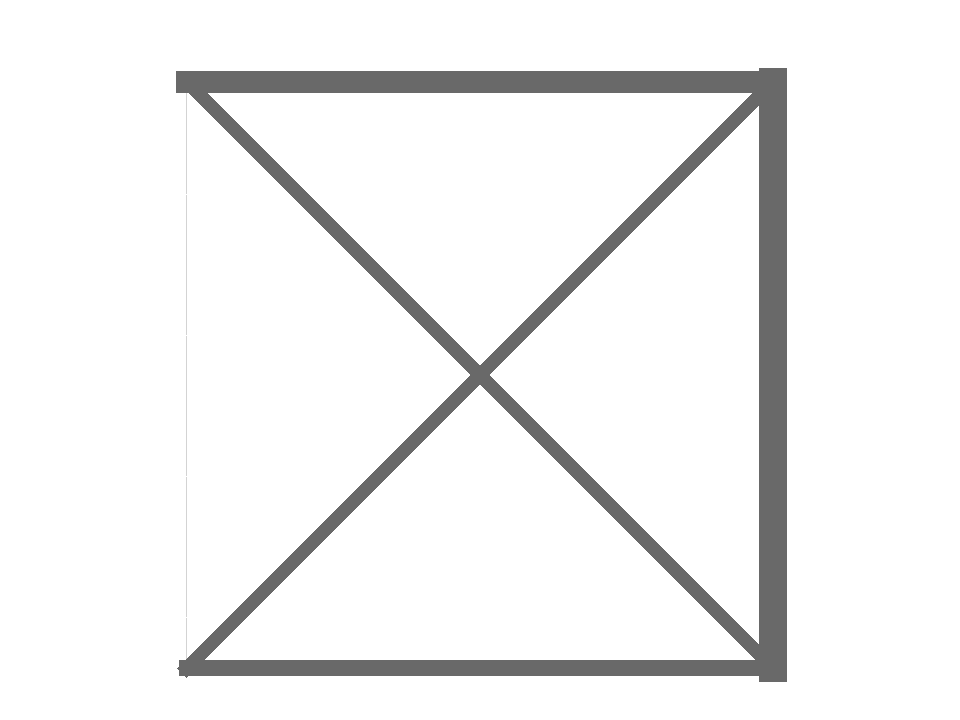
\includegraphics[width=0.3\linewidth]{figures/06_DMO/00_optimized_module/fig8-Module_Topology_001.pdf}}
    \hspace*{\fill}
    \caption{}
    \label{fig:06}
\end{figure}
\todo{tables with volume and phi and psi for different NT}

\begin{figure}
    \centering
    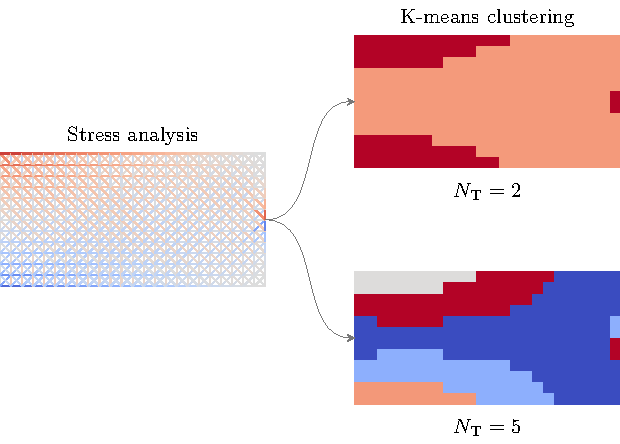
\includegraphics{figures/06_DMO/00_optimized_modules/kmeans.pdf}
    \caption{}
    \label{fig:06}
\end{figure}

\begin{figure*}
    \subcaptionbox{}{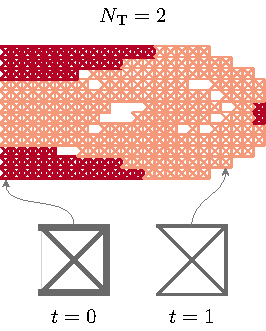
\includegraphics[width=0.3\linewidth]{figures/06_DMO/00_optimized_modules/nt2.pdf}}
    \hfill
    \subcaptionbox{}{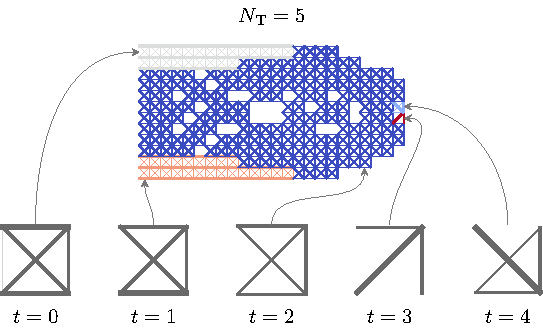
\includegraphics[width=0.6\linewidth]{figures/06_DMO/00_optimized_modules/nt5.pdf}}
    \caption{}
    \label{fig:06}
\end{figure*}

\subsection{A benchmark case study: a simply supported modular bridge}

\begin{figure}
    \centering
    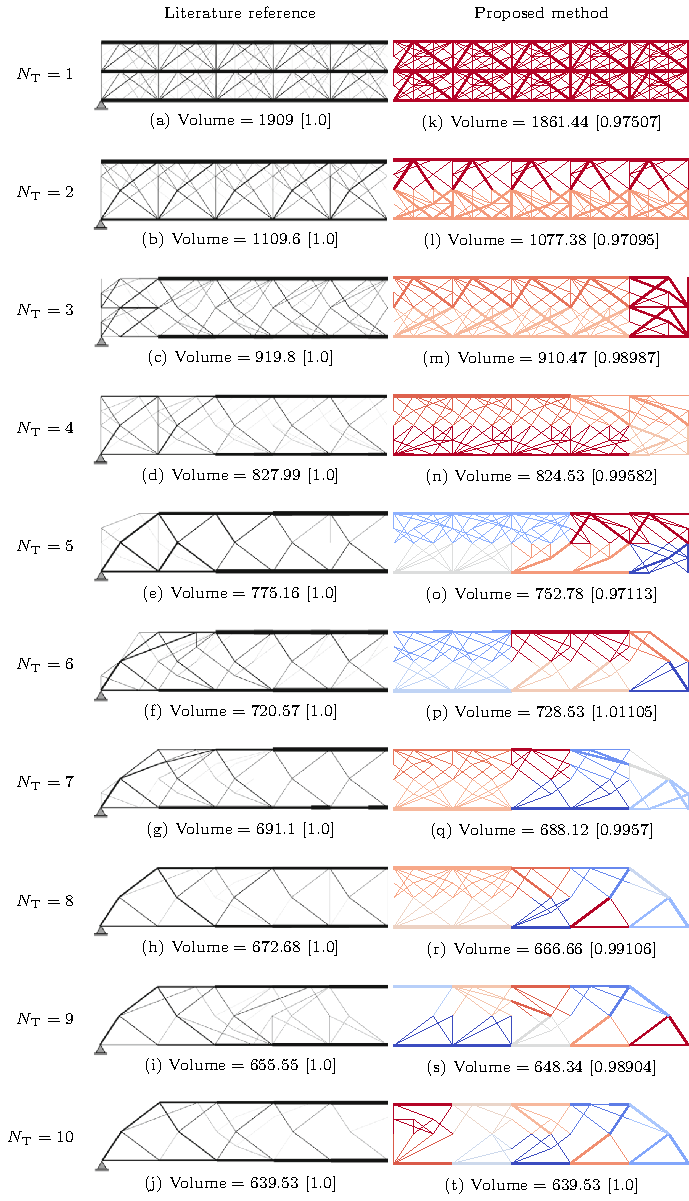
\includegraphics{figures/06_DMO/00_tug_bench/bench.pdf}
    \caption{}
    \label{fig:06}
\end{figure}

\begin{figure}
    \centering
    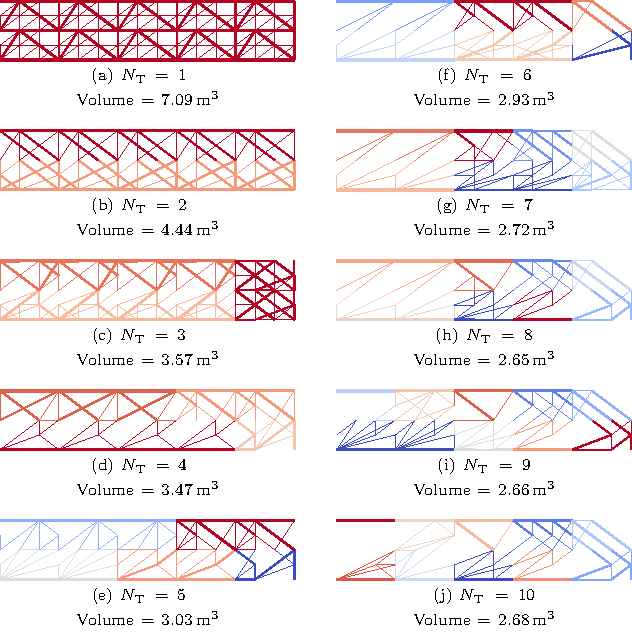
\includegraphics{figures/06_DMO/00_tug_bench_buck/buck.pdf}
    \caption{}
    \label{fig:06}
\end{figure}

\subsection{On the importance of the local buckling}

\subsection{Simply supported 3D beam}
\begin{margintable}
    \small
    \centering
    \begin{tabular}{cc}
    \toprule
    \textbf{Parameter}        & \textbf{Value} \\ \midrule
    $E$              & \qty{2.7}{GPa}     \\
    $\nu$            & 0.3   \\
    $\sigma_\text{c}, \sigma_\text{t}$ & $\pm $\qty{55}{MPa} \\
    $\rho$              & \qty{1.14}{\gram\per\cubic\centi\metre}   \\
    $P$              & \qty{100}{N}   \\
    \bottomrule
    \end{tabular}
    \caption{Material data used for the simply supported 3D beam optimization.}
    \label{tab:06_3D_supp_mat}
\end{margintable}


\section{Conclusion}